 \documentclass{article}
\usepackage{amsmath}
\usepackage{hyperref}
\usepackage{graphicx}
\usepackage{adjustbox}
\newcommand{\tabincell}[2]{\begin{tabular}{@{}#1@{}}#2\end{tabular}}

\begin{document} %This is where document begins
\begin{titlepage}
\title{EE 232E \\Graphs and Network Flows\\Homework 1\\Winter 2016} 
\author{Liqiang Yu, Rongjing Bai, Yunwen Zhu\\
904592975, 204587519, 104593417}  %change your ID here
\date{04-12-2016}
\end{titlepage}

\maketitle
\newpage
\tableofcontents
\newpage

\section{Problem1}\label{prob:p1}
In this part, we create random networks with probability p for drawing an edge between two arbitrary vertices and discussion the relationship between p and connectedness of the graph.
\subsection{Part a}
(i) when p = 0.01, we can get the degree distribution in Figure \ref{fig:p1_1}.
\begin{figure}[htbp]
\centering
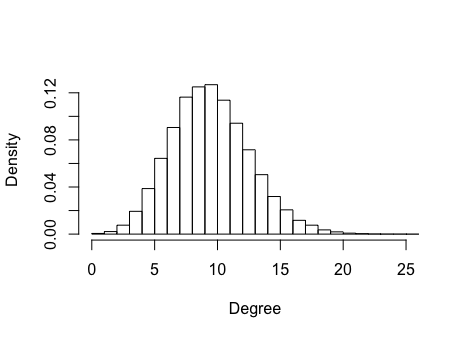
\includegraphics[width=.6\textwidth]{p1_1.png}
\caption{The degree distribution for p = 0.01}
\label{fig:p1_1}
\end{figure}\\
\\
(ii) when p = 0.05, we can get the degree distribution in Figure \ref{fig:p1_2}.
\begin{figure}[htbp]
\centering
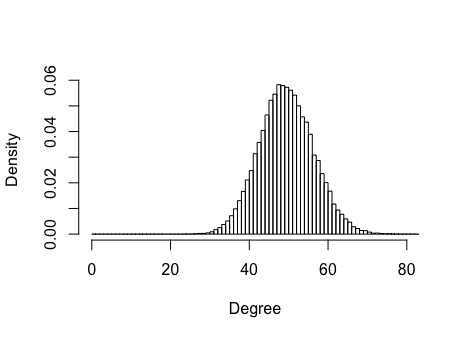
\includegraphics[width=.6\textwidth]{p1_2.png}
\caption{The degree distribution for p = 0.05}
\label{fig:p1_2}
\end{figure}\\
\\
(iii) when p = 0.1, we can get the degree distribution in Figure \ref{fig:p1_3}.
\begin{figure}[htbp]
\centering
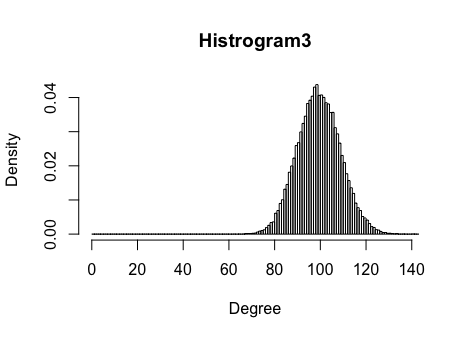
\includegraphics[width=.6\textwidth]{p1_3.png}
\caption{The degree distribution for p = 0.1}
\label{fig:p1_3}
\end{figure}\\
\\
Based on the three figures, we can see that as the probability for drawing an edge between two arbitrary vertices increases, the degree increases conrespondingly, which conforms to our thought. 
\subsection{Part b}
To check whether or not these network are connected and the diameter of these networks, we use is.connected() and diameter()function. And as this is the random network, we run the test for 50 times to get a more accurate result. Thus, in this way, we get the ratio of whether the network is connected and average diameter of the networks. The results are shown in Table \ref{tb:p1_b}.
\begin {table}[htbp]
\caption{parameters of random network}
\begin{adjustbox}{center}
\label{tb:p1_b}
\begin{tabular}{|c|c|c|c|}
\hline
\tabincell{c}{} & p = 0.01 & p = 0.05 & p = 0.1\\
\hline
\tabincell{c}{ratio of connectedness}&0.9&1&1\\
\hline
\tabincell{c}{diameter}&5.4&3&3\\
\hline
\end{tabular}
\end{adjustbox}
\end{table}\\
\\
Based on the results, we can see that the network has a rather high ration of connectedness. Thus, all of these networks can be regarded as connected.
\subsection{Part c}
In order to find out the value of $p_{c}$, we start from the small value of p until the network become connected. And as this is the random network, we run the test for 100 times to get a more accurate result. Thus, in this way, we get $p_{c}$ =  0.006371, which roughly corresponds to the value in theory.
\section{Problem2}
\subsection{Part a}
The average diameter of network is 20 after we run 100 times, and its degree distribution is shown in figure \ref{fig:p2_1}
\begin{figure}[htbp]
\centering
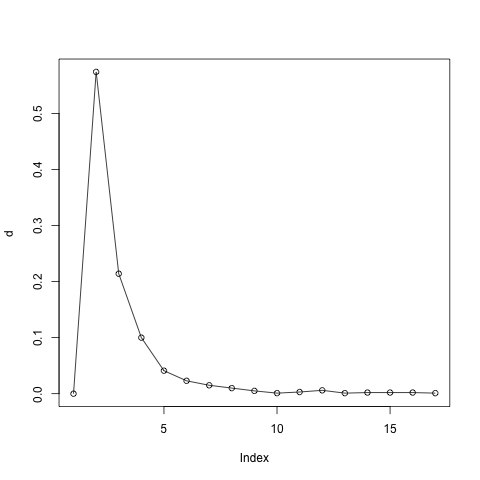
\includegraphics[width=.6\textwidth]{p2_1.png}
\caption{The distribution for fat tailed graph}
\label{fig:p2_1}
\end{figure}

\subsection{Part b}
We repeated 100 times the graph is always connected.
The GCC is the whole graph.
Number of communities (best split) is 34.
The modularity is 0.9348964.\\
\\
The value of modularity is very big because connections between nodes in different modules are sparse, but between nodes in same modules are dense. 
\subsection{Part c}
When we build a graph with 10000 nodes, the best split number of community is 105 and the corresponding modularity becomes 0.9792582.
It is greater than the modularity of the case with 1000 nodes.
\subsection{Part d}
We use histogram to describe the degree distribution. The result is shown in figure \ref{fig:p2_2}. \\
\begin{figure}[htbp]
\centering
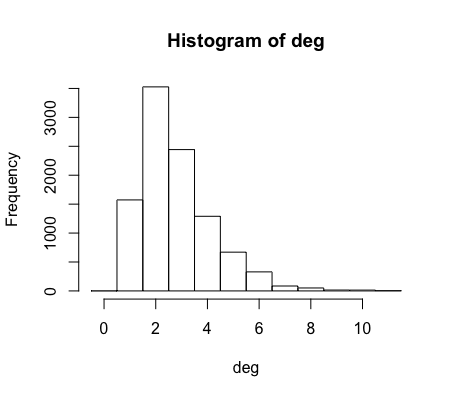
\includegraphics[width=.6\textwidth]{p2_2.png}
\caption{The distribution histogram of degreel}
\label{fig:p2_2}
\end{figure}
\\
\\
From the graph we can see that, the most common degree is 2.
\section{Problem 3}
\subsection{Part a}
We create a evolving random undirected graph with 1000 nodes, the preferantial attachment exponent is 1, the aging exponent is 0 and the number of bins is 1000. The degree distribution is shown in figure \ref{fig:p3_1}.
\begin{figure}[htbp]
\centering
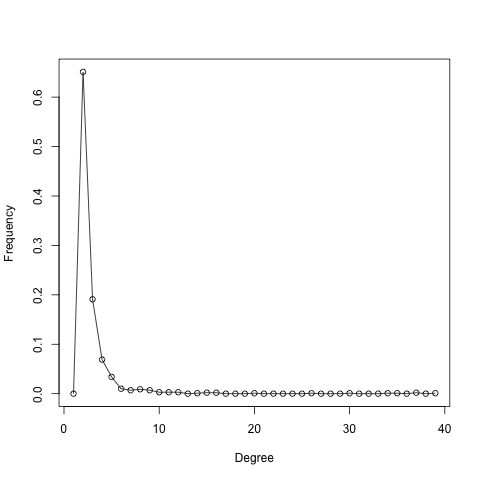
\includegraphics[width=.6\textwidth]{p3_1.png}
\caption{The degree distribution for evolving random graph}
\label{fig:p3_1}
\end{figure}
\subsection{Part b}
In order to calculate the modularity, we used the fast greedy algorithm. We ran the test for 100 times and calculated the average of modularity, the average modularity is 0.9225776. One of the community structure is shown in figure \ref{fig:p3_2}.
\begin{figure}[htbp]
\centering
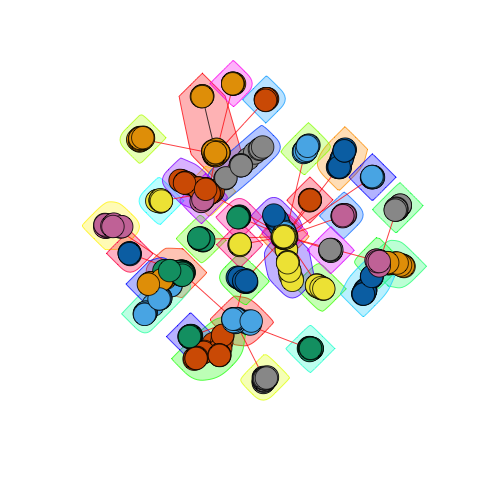
\includegraphics[width=.8\textwidth]{p3_2.png}
\caption{The community structure of the graph}
\label{fig:p3_2}
\end{figure}
\section{Problem 4}
\subsection{Part a}
In this part, we used the forest fire model to simulate a growing network. The network contained 1000 nodes. Again, we ran the test for 100 times and calculated the avarage input and output degree distribution. Figure \ref{fig:in} shows the input degree distribution and figure \ref{fig:out} shows the output degree distribution. The figure \ref{fig:inout} shows the result if we put the input and output degree in the same image, from which we can see that the input degree is approximately equal to the output degree.
\begin{figure}[htbp]
\centering
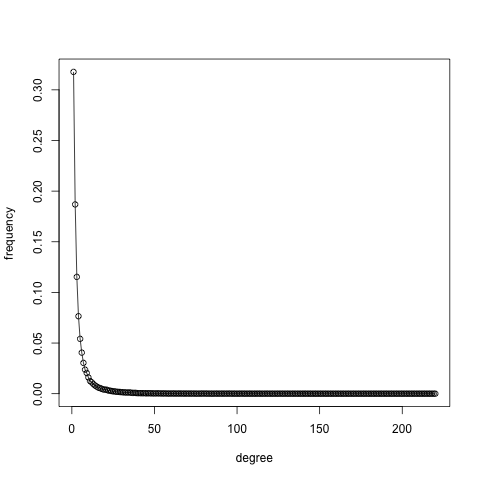
\includegraphics[width=.6\textwidth]{degree_in.png}
\caption{The input degree distribution}
\label{fig:in}
\end{figure}

\begin{figure}[htbp]
\centering
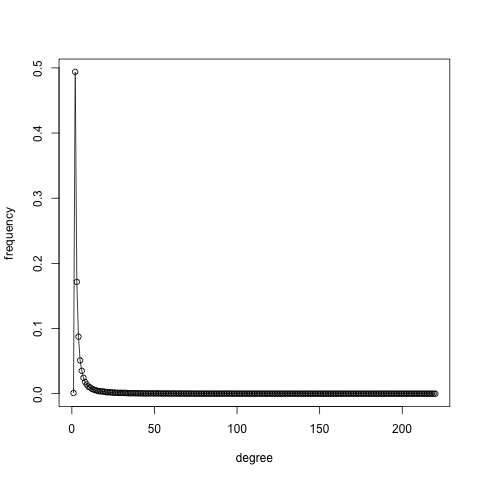
\includegraphics[width=.6\textwidth]{degree_out.png}
\caption{The output degree distribution}
\label{fig:out}
\end{figure}

\begin{figure}[htbp]
\centering
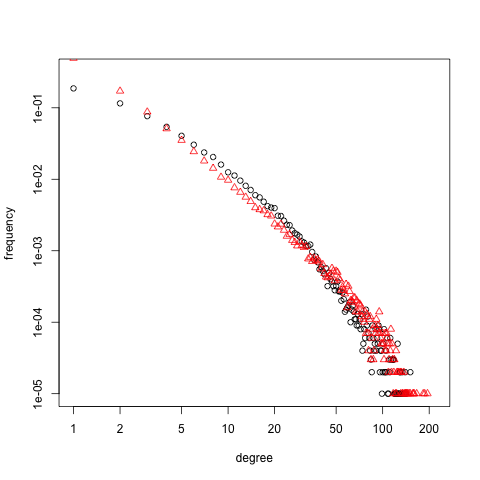
\includegraphics[width=.6\textwidth]{in_out.png}
\caption{The intput and output degree distribution}
\label{fig:inout}
\end{figure}
\subsection{Part b}
We calculated the avarage diameter of the graph through 100 test and the diameter result is 10.46.
\subsection{Part c}
We chose to use random walks algorithm to calculate the community because it is more fit for directed graph. The tests were also run for 100 times and one of the community structures is shown in figure \ref{fig:com} and the average modularity is 0.42.
\begin{figure}[htbp]
\centering
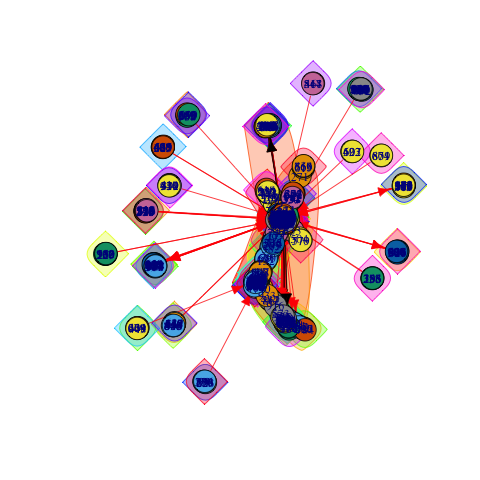
\includegraphics[width=.8\textwidth]{p4.png}
\caption{The community structure of the growing graph}
\label{fig:com}
\end{figure}

\end{document}
